\textbf{Тема:} Программная реализация приближенного аналитического метода и численных алгоритмов первого и второго порядков точности при решении задачи Коши для ОДУ.

\textbf{Цель работы.} Получение навыков решения задачи Коши для ОДУ методами Пикара и явными методами первого порядка точности (Эйлера) и второго порядка точности (Рунге-Кутта).

\textbf{Исходные данные.}
\begin{enumerate}
    \item ОДУ, не имеющее аналитического решения
    \begin{equation*}
        \begin{cases}
            u'(x) = x^2 + u^2, \\
            u(0) = 0,
        \end{cases}
    \end{equation*}
\end{enumerate}

\textbf{Результаты работы программы}

Таблица, содержащая значения аргумента с заданным шагом в интервале $[0, x_{max}]$ и
результаты расчета функции $u(x)$ в приближениях Пикара (от 1-го до 4-го), а также
численными методами. Границу интервала $x_{max}$ выбирать максимально возможной из условия, чтобы численные методы обеспечивали точность вычисления решения уравнения
$u(x)$ до второго знака после запятой.

\textbf{Вопросы при защите лабораторной работы}
\begin{enumerate}
    \item Укажите интервалы значений аргумента, в которых можно считать решением заданного уравнения каждое из первых 4-х приближений Пикара. Точность результата оценивать до второй цифры после запятой. Объяснить свой ответ.
    \item Пояснить, каким образом можно доказать правильность полученного результата при фиксированном значении аргумента в численных методах.
    \item Каково значение функции при $x=2$, т.е. привести значение $u(2)$.
\end{enumerate}

\section{Метод Пикара}
Метод Пикара является представителем приближенных методов решения рассматриваемого класса задач. Идея метода сводится к процедуре последовательных приближений для решения интегрального уравнения, к которому приводится исходное дифференциальное уравнение.

Поставлена задача Коши:
\eq{
    \begin{cases}
        u'(x) = f(x, u(x)), \\
        u(x_0) = u_0
    \end{cases}
}

Проинтегрируем выписанное уравнение
\eq{u(x) = u_0 + \int_{x_0}^{x} f(t,u(t)) \,dt \ }

Процедура последовательных приближений метода Пикара реализуется согласно следующей схеме
\eq{ y_s(x) = u_0 + \int_{x_0}^{x} f(t,y_{s-1}(t)) \,dt \ , }
причем $y_0(t) = v_0$, (i – номер итерации).

Заданная в лабораторной работе ОДУ, не имеющее аналитического решения
\eq{
    \begin{cases}
        u'(x) = x^2 + u^2, \\
        u(0) = 0,
    \end{cases}
}

Правая часть непрерывна и удовлетворяет условию Липшица. Значит, решение существует, а метод Пикара сойдется. По схеме Пикара рассчитаем первые четыре приближения для заданного ОДУ.
\eq{y_1(x) = 0 + \int_{0}^{x} t^2 \,dt \  = \frac{x^3}{3}}
\eq{y_2(x) = 0 + \int_{0}^{x} (t^2  + (\frac{t^3}{3})^2) \,dt \  = \frac{x^3}{3} + \frac{x^7}{63}}
\eq{y_3(x) = 0 + \int_{0}^{x} (t^2  + (\frac{t^3}{3} + \frac{t^7}{63})^2) \,dt \  = \frac{x^3}{3} + \frac{x^7}{63} + \frac{2x^{11}}{2079} + \frac{x^{15}}{59535}}
\eq{\begin{gathered}
    	y_4(x) = 0 + \int_{0}^{x} (t^2  + (\frac{t^3}{3} + \frac{t^7}{63} + \frac{2t^{11}}{2079} + \frac{t^{15}}{59535})^2) \,dt \ = \\ = \frac{x^3}{3} + \frac{x^7}{63} + \frac{2x^{11}}{2079} + \frac{13x^{15}}{218295} + \frac{82x^{19}}{37328445} + \frac{662x^{23}}{10438212015} + \frac{4x^{27}}{3341878155} + \frac{x^{31}}{109876902975}
    \end{gathered}}

\section{Метод Эйлера}
Также задача может быть решена с помощью численных методов. 
\eq{y_{n + 1} = y_n + hf(x_n, y_n)}
\eq{f(x_n, y_n) = y_n^2 + x_n^2}


\section{Метод Рунге-Кутта 2-ого порядка точности}
\begin{equation}
	y_{n+1} = y_n + h[(1 - \alpha) k_1 + \alpha k_2],
	\label{eq_rungre:ref}
\end{equation}
где  
\eq{k_1 = f(x_n, y_n),}
\eq{k_2 = f(x_n + \frac{h}{2\alpha}, y_n + \frac{h}{2\alpha}k_1),}
В практике расчетов используют формулу \eqref{eq_rungre:ref} при значениях $\alpha = 1$, $\alpha = \frac{1}{2}$. В лабораторной работе приняли $\alpha = \frac{1}{2}$
\section{Листинг программы}
\begin{lstlisting}
import java.lang.Math.pow
import kotlin.math.abs

fun f(x: Double, y: Double): Double {
    return pow(x, 2.0) + pow(y, 2.0);
}

val picardOne: (x: Double) -> Double = {
        x -> pow(x, 3.0) / 3
}
val picardTwo: (x: Double) -> Double = {
        x -> picardOne(x) +
        pow(x, 7.0) / 63
}
val picardThree: (x: Double) -> Double = {
        x -> picardTwo(x) +
        2 * pow(x, 11.0) / 2079 +
        pow(x, 15.0) / 59535
}
val picardFour: (x: Double) -> Double = {
        x -> picardThree(x) +
        4 * pow(x, 15.0) / 93555 +
        82 * pow(x, 19.0) / 37328445 +
        662 * pow(x, 23.0) / 10438212015 +
        4 * pow(x, 27.0) / 3341878155 +
        pow(x, 31.0) / 109876902975
}

fun picard(columnX: ArrayList<Double>,
           funcPickard: (x: Double)-> Double): ArrayList<Double> {
    var columnY = arrayListOf<Double>()
    for (x in columnX) {
        val y = funcPickard(x)
        columnY.add(y)
    }
    return  columnY
}

fun euler(columnX: ArrayList<Double>, h:Double): ArrayList<Double> {
    var columnY = arrayListOf<Double>()
    var y = 0.0
    for (x in columnX) {
        y += h * f(x, y)
        columnY.add(y)
    }
    return  columnY
}

fun runge(columnX: ArrayList<Double>, h:Double): ArrayList<Double> {
    var columnY = arrayListOf<Double>()
    var y = 0.0
    val alpha = 0.5

    for (x in columnX) {
        val k1 = f(x, y)
        val k2 = f(x + h / 2 / alpha, y + k1 * h / 2 / alpha)
        y += h * ((1 - alpha) * k1 + alpha * k2)
        columnY.add(y)
    }
    return  columnY
}

fun printColumns(table: ArrayList<ArrayList<Double>>, eps:Double) {
    var i = 0
    while (abs(table[6][i] - table[5][i]) <= eps) {
        print("| %4.3f   ".format(table[0][i]))

        for (j in 1..(table.size - 1)) {
            print("| %7.6f    ".format(table[j][i]))
        }
        println("| %4.3f       |".format(abs(table[6][i] - table[5][i])))
        i++
    }
    println("-".repeat(109))
}

fun printHead() {
    var line = "-".repeat(109)
    println(line)
    println("|         |                       Метод Пикара                    " +
            "|  Метод      |    Метод    |             |")
    println("|   x     |      1      |      2      |      3      |      4      " +
            "|  Эйлера     | Рунге-Кутта |  Точность   |")
    println(line)

}

fun printTable(table: ArrayList<ArrayList<Double>>, eps: Double) {
    printHead()
    printColumns(table, eps)

}

fun getX(firstX: Double, maxX: Double, h: Double): ArrayList<Double> {
    var columnX = arrayListOf<Double>()
    var x = firstX
    while(x <= maxX) {
        columnX.add(x)
        x += h
    }
    return columnX
}

fun main() {
    val firstX = 0.0
    val maxX = 2.0
    val h = 0.01
    val eps = 0.01

    println("Начальный x = " + firstX)
    println("Максимальный x = " + maxX)
    println("Шаг для численных методов = " + h)
    println("Точность Eps = " + eps)

    var table = arrayListOf<ArrayList<Double>>()
    val columnX = getX(firstX, maxX, h)
    table.add(columnX)
    table.add(picard(columnX, picardOne))
    table.add(picard(columnX, picardTwo))
    table.add(picard(columnX, picardThree))
    table.add(picard(columnX, picardFour))
    table.add(euler(columnX, h))
    table.add(runge(columnX, h))
    printTable(table, eps)
}
\end{lstlisting}

\section{Результаты работы программы}
На рисунках представлены результаты работы программы. Вывод таблицы осуществляется, пока численные методы обеспечивают точность вычисления решения уравнения $u(x)$ до второго знака после запятой.
\begin{figure}[h!]
\center{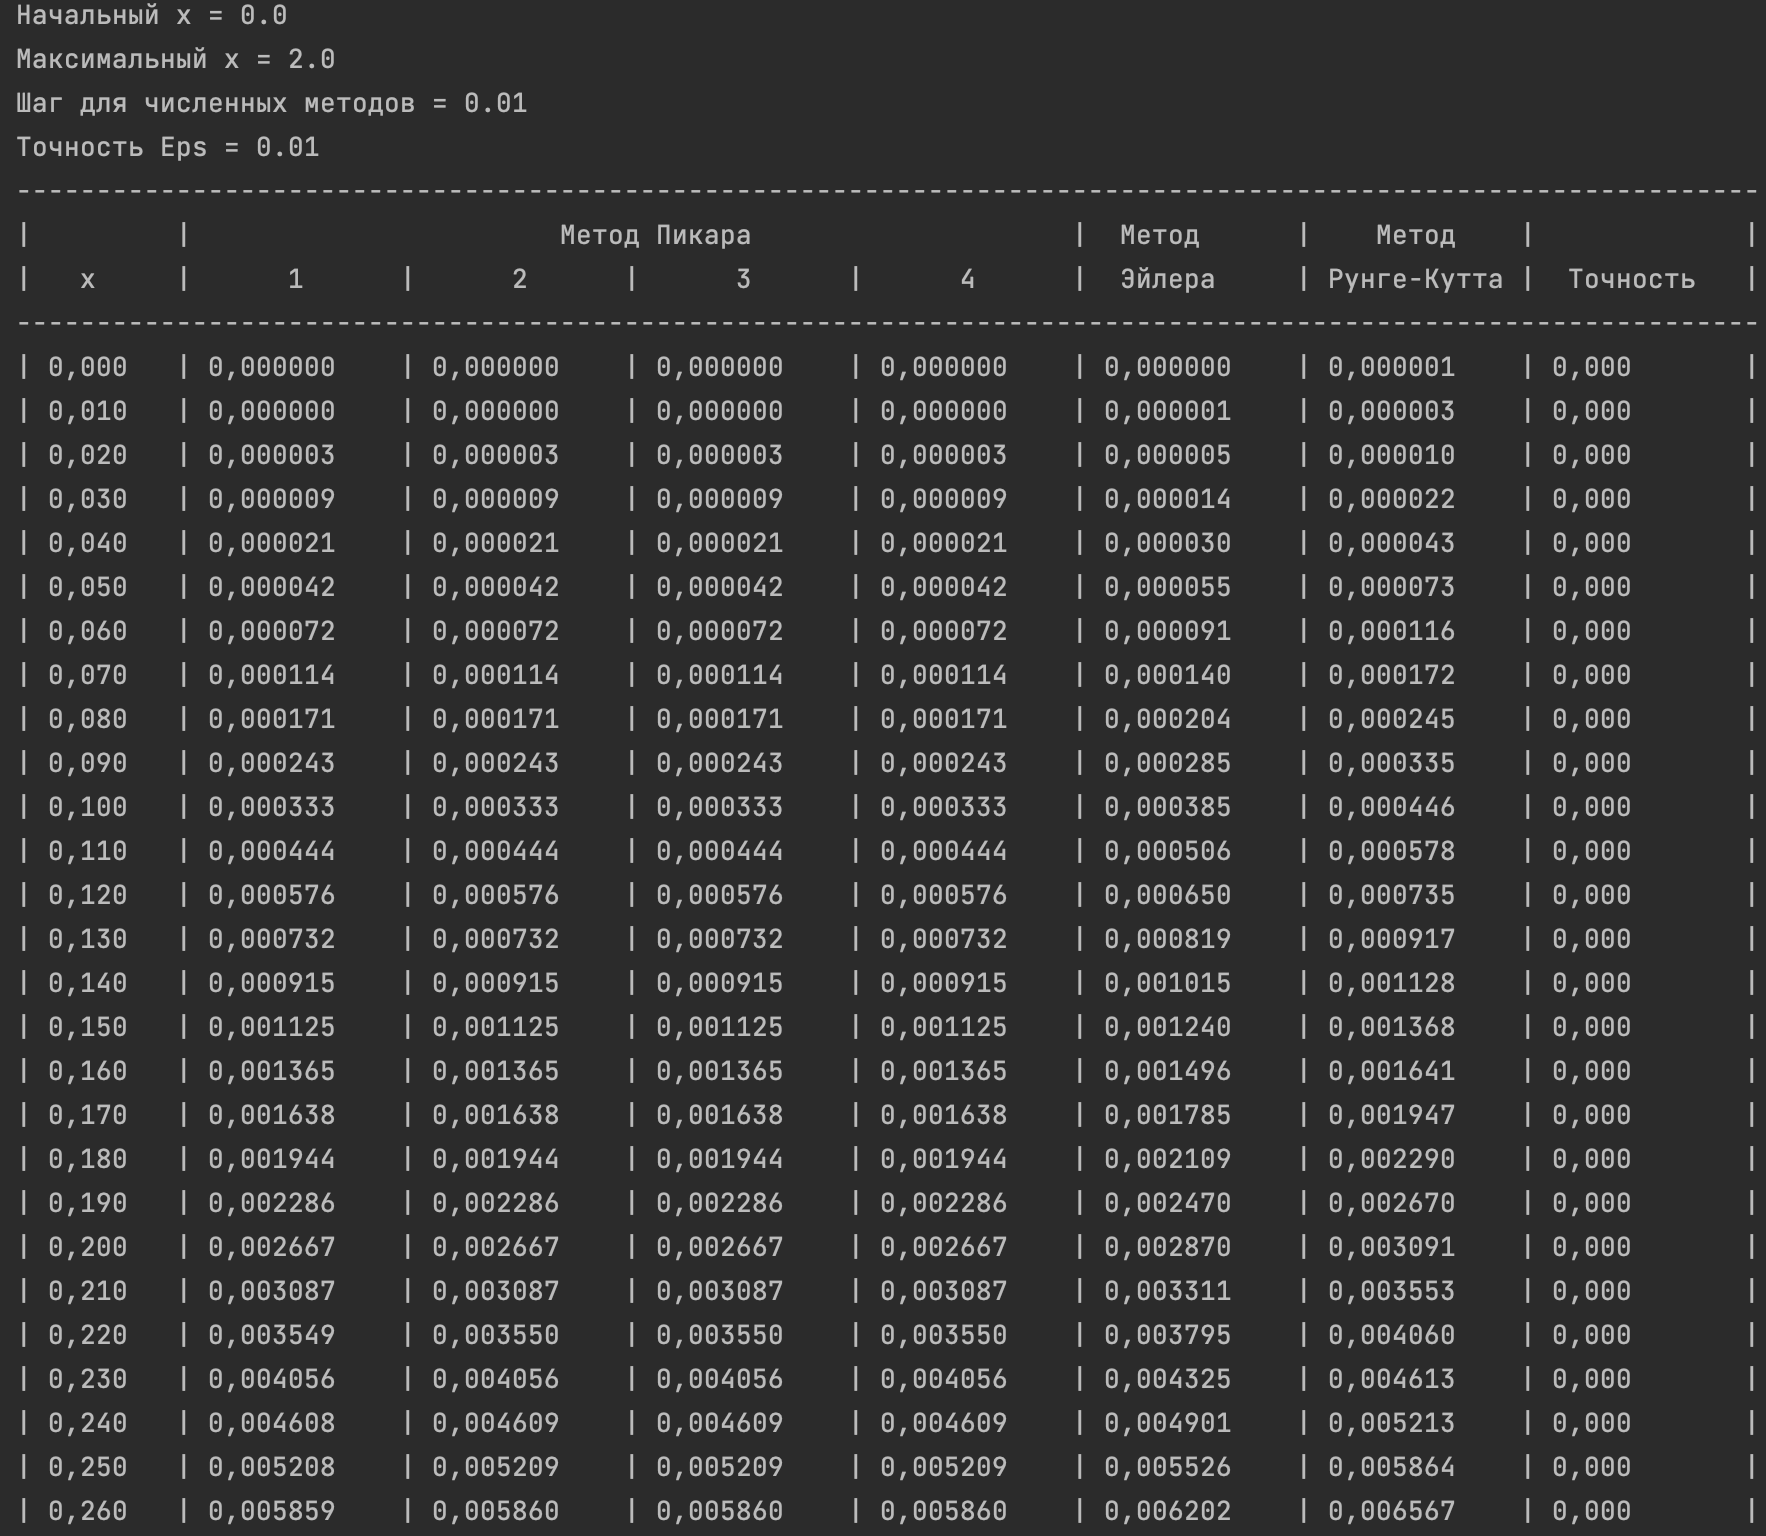
\includegraphics[scale=0.35]{fig/pic01.png}}
\caption{Результаты работы программы}
\end{figure}
\begin{figure}[h!]
\center{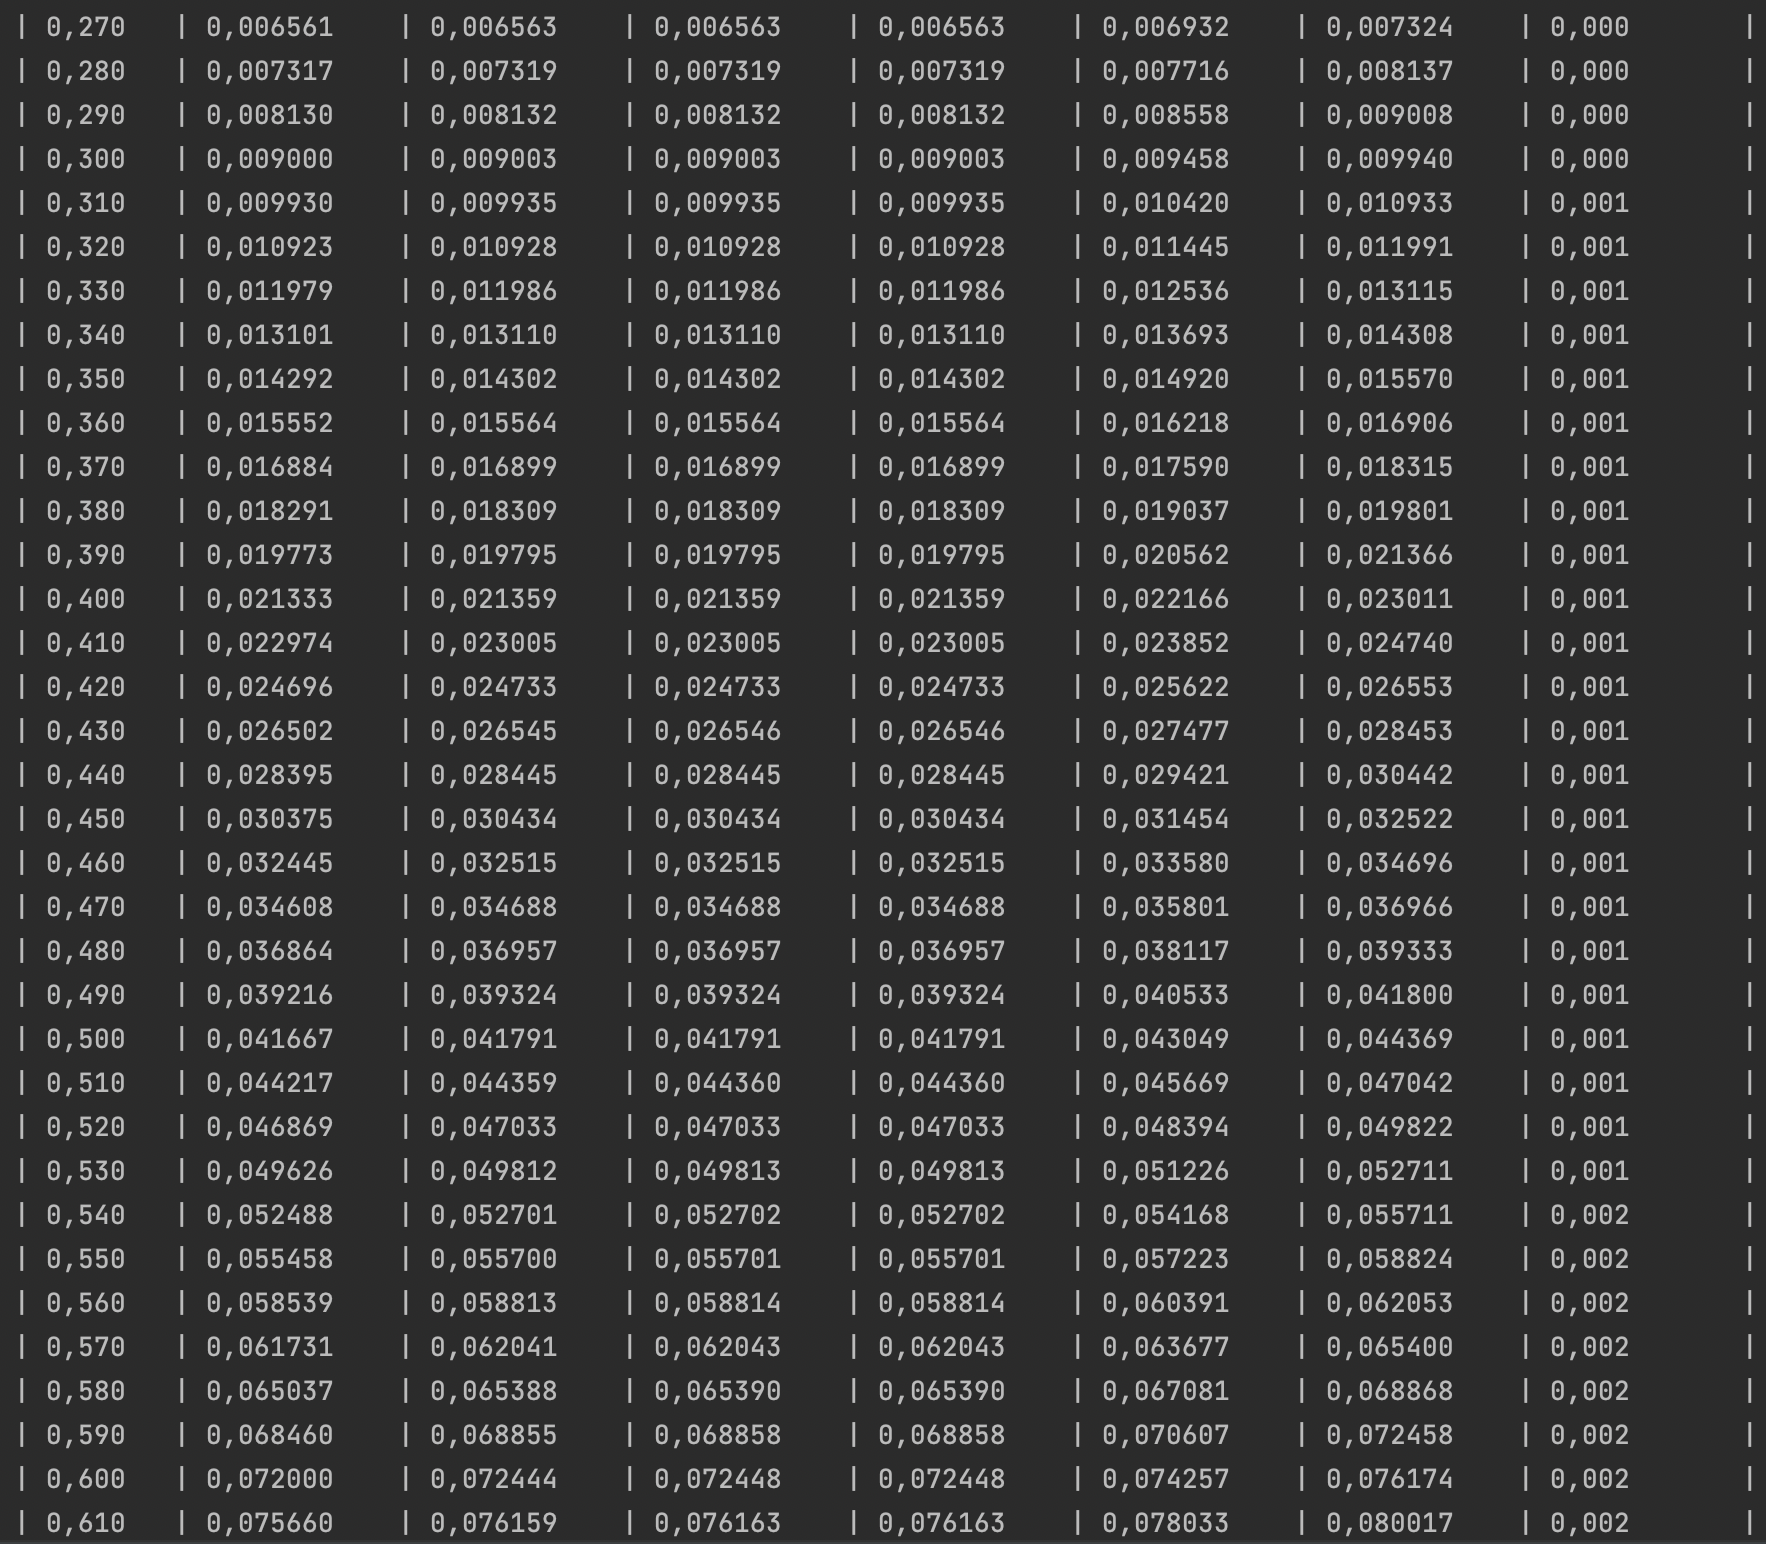
\includegraphics[scale=0.37]{fig/pic02.png}}
\caption{Результаты работы программы (продолжение)}
\label{ris:image}
\end{figure}
\begin{figure}[h!]
\center{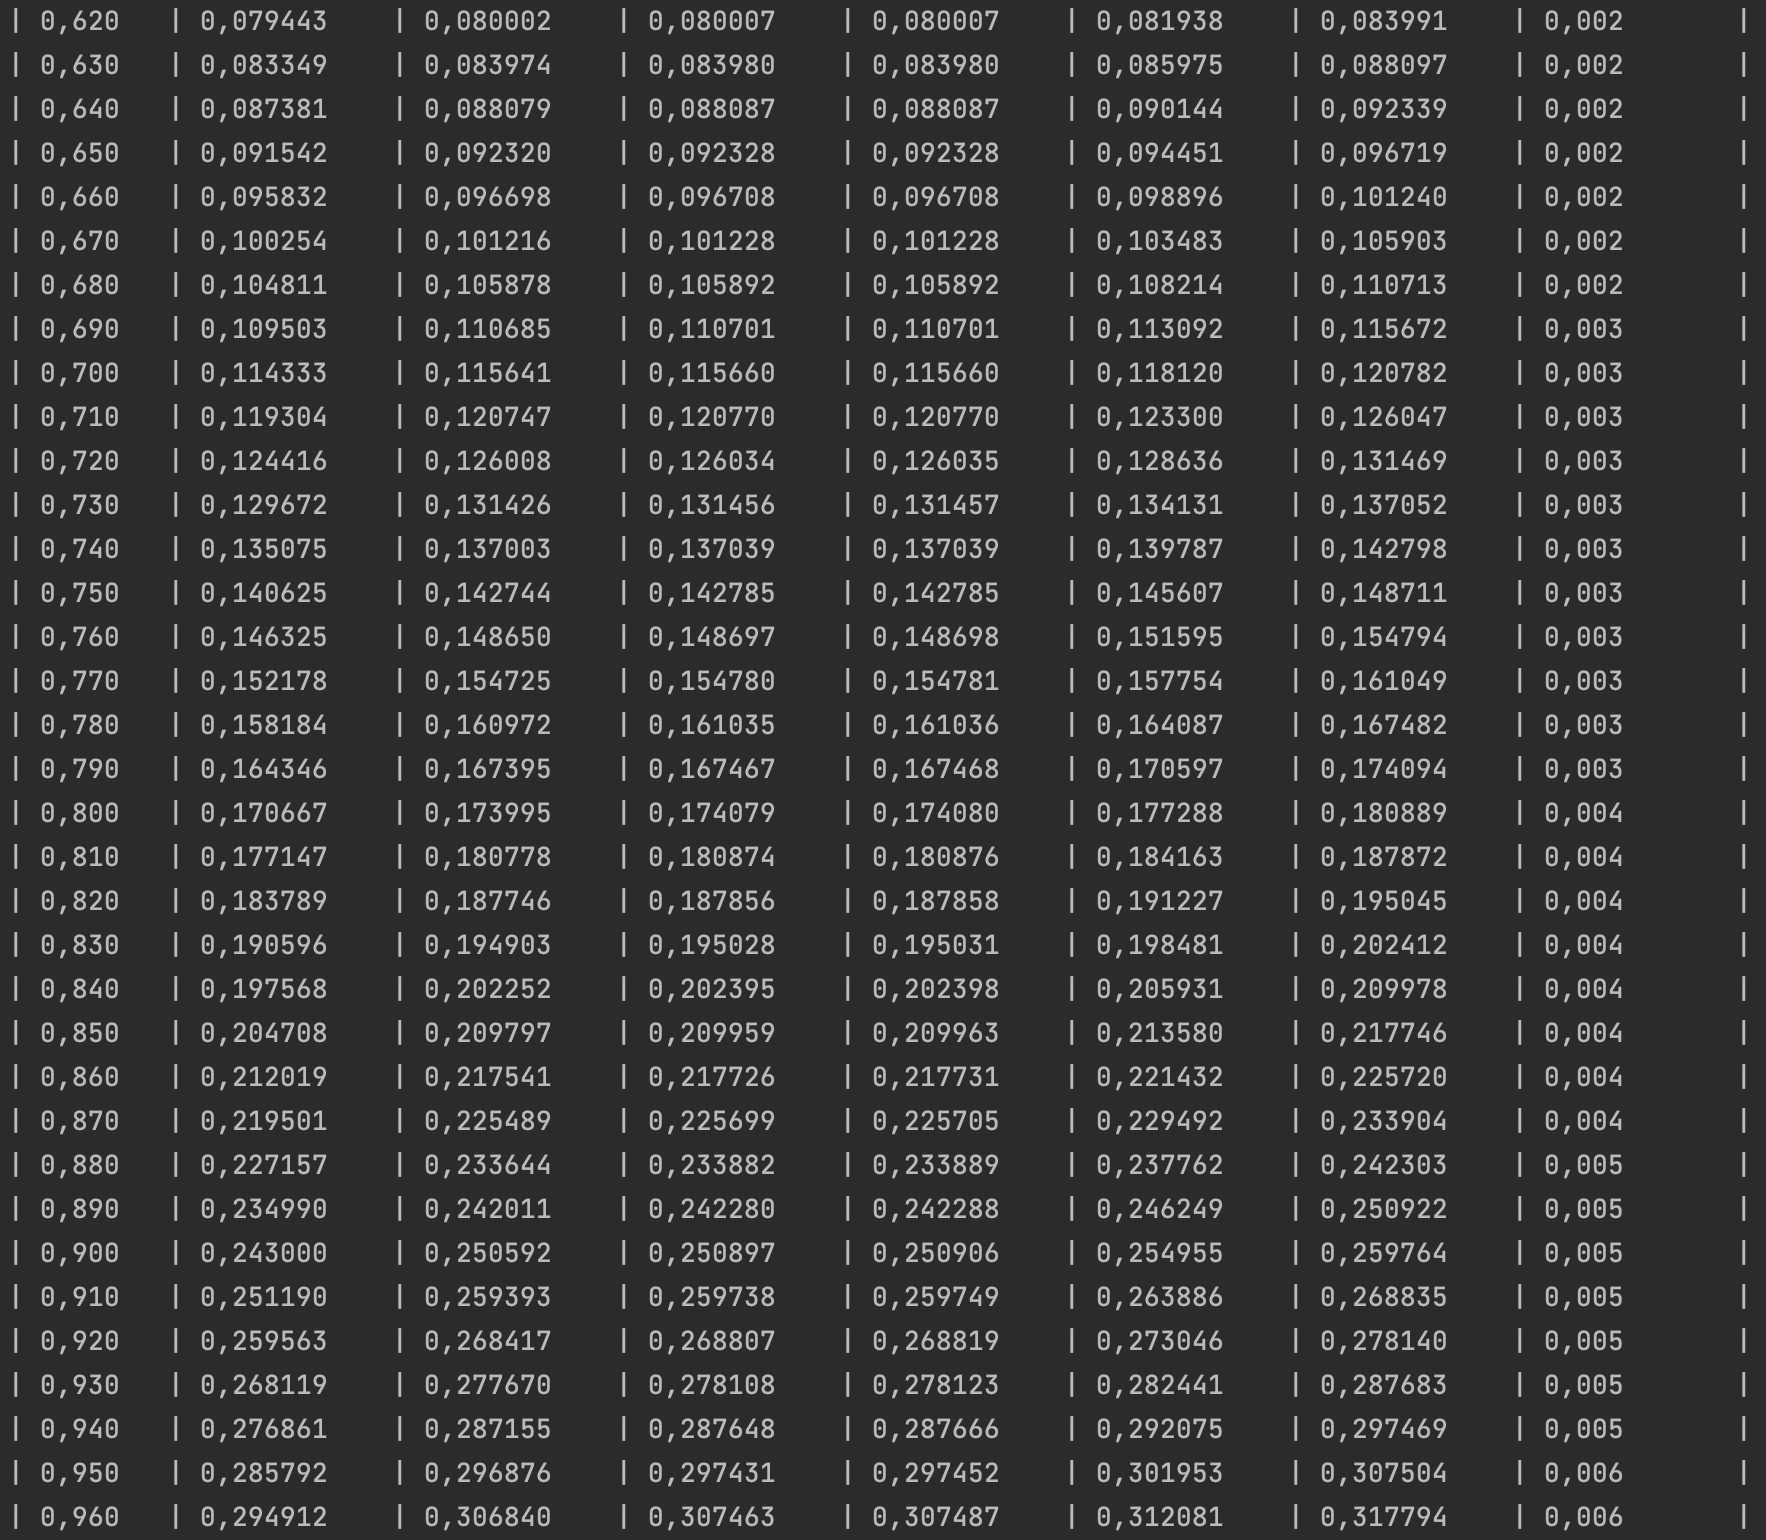
\includegraphics[scale=0.37]{fig/pic03.png}}
\caption{Результаты работы программы (продолжение)}
\label{ris:image}
\end{figure}
\begin{figure}[h!]
\center{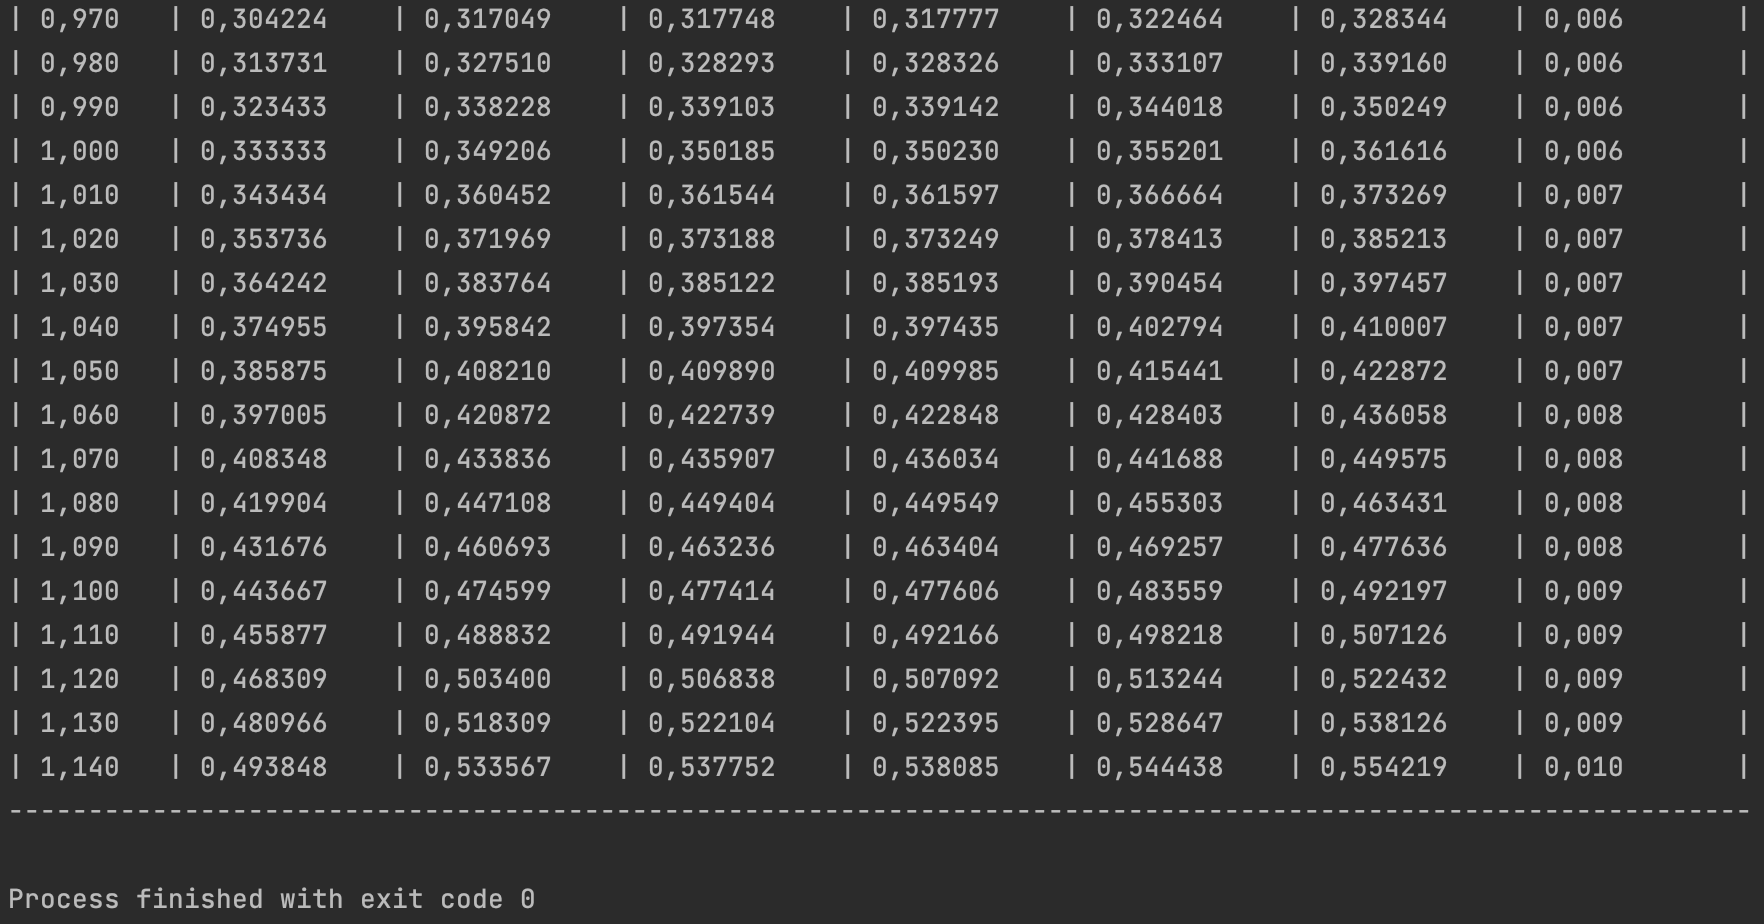
\includegraphics[scale=0.37]{fig/pic04.png}}
\caption{Результаты работы программы (продолжение)}
\label{ris:image}
\end{figure}
\newline
\newpage
\newpage
\section{Ответы на вопросы}
\begin{enumerate}
    \item \textbf{Укажите интервалы значений аргумента, в которых можно считать решением заданного уравнения каждое из первых 4-х приближений Пикара. Точность результата оценивать до второй цифры после запятой. Объяснить свой ответ.}
    
    Каждое следующее приближение Пикара точнее предыдущего. n-ое приближение Пикара можно считать решением уравнения, если выполняется условие 
    \eq{|y_n(x) - y_{n+1}(x)| < \epsilon,}
    Для вычисления интервала 4-ого приближения нужно рассчитать 5-ое приближение. \newline
    Листинг программы:
    \begin{lstlisting}
fun main() {
    val firstX = 0.0
    val maxX = 2.0
    val h = 0.001
    val eps = 0.01

    var table = arrayListOf<ArrayList<Double>>()
    val columnX = getX(firstX, maxX, h)
    table.add(columnX)
    table.add(picard(columnX, picardOne))
    table.add(picard(columnX, picardTwo))
    table.add(picard(columnX, picardThree))
    table.add(picard(columnX, picardFour))

    var i = 0
    while(abs(table[2][i] - table[1][i]) <= eps) i++
    println("Для 1- ого приближения x принадлежит [0, %4.3f".format(table[0][i]) + "]")
    while(abs(table[3][i] - table[2][i]) <= eps) i++
    println("Для 2- ого приближения x принадлежит [0, %4.3f".format(table[0][i]) + "]")
    while(abs(table[4][i] - table[3][i]) <= eps) i++
    println("Для 3- его приближения x принадлежит [0, %4.3f".format(table[0][i]) + "]")
}
    \end{lstlisting}
    \textbf{Результаты работы программы:}
    При заданной точности $\epsilon = 0.01$ n-е приближение Пикара является решением, когда x принадлежит интервалам:
    \begin{figure}[h!]
        \center{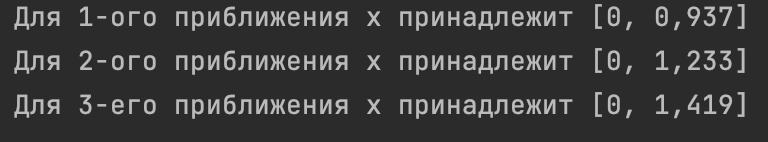
\includegraphics[scale=0.6]{fig/pic05.png}}
        \caption{Результаты работы программы (задание 1)}
    \end{figure}
    \newline\newline\newline
    \item \textbf{Пояснить, каким образом можно доказать правильность полученного результата при фиксированном значении аргумента в численных методах.}
    
     Точность численных методов зависит от шага, поэтому чтобы доказать правильность полученного результата при фиксированном значении аргумента в численных методах, нужно сравнить полученное значение со значением, полученном при меньшем шаге. 
    \item \textbf{Каково значение функции при $x=2$, т.е. привести значение $u(2)$.}
    
    По схеме ответа на вопрос №2 рассчитаем значение $u(2)$
    
    $u(2) = 317.72$
    \begin{lstlisting}
fun getEuler(firstX:Double, maxX:Double, firstY: Double, h:Double):Double {
    var x = firstX
    var y = firstY
    while (x <= maxX) {
        y += h * f(x, y)
        x += h
    }
    return  y
}

fun main(){
    val firstX = 0.0
    val maxX = 2.0
    var h = 0.1
    val eps = 0.01
    val firstY = 0.0

    var curY = 0.0
    var nextY = getEuler(firstX, maxX, firstY, h)
    println("     h      |      u(2)     |  точность")
    do {
        curY = nextY
        h *= 0.1
        nextY = getEuler(firstX, maxX, firstY, h)
        println("%1.9f | %13.9f | %1.3f".format(h*10, curY, abs(nextY - curY)))
    } while(abs(curY - nextY) > eps)

    println("u(2) = " + curY)
}
    \end{lstlisting}
     \begin{figure}[h!]
        \center{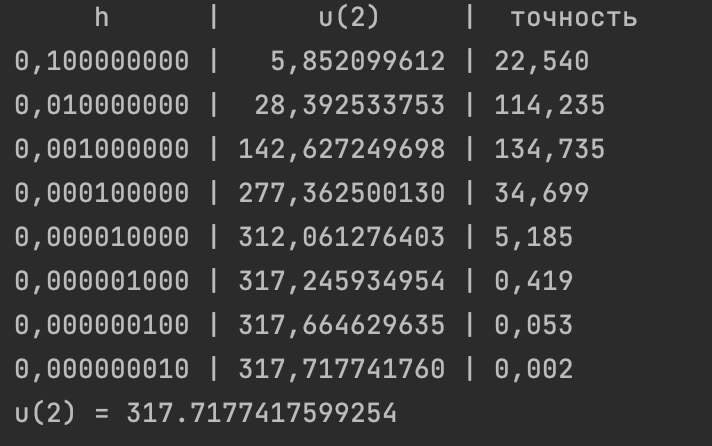
\includegraphics[scale=0.6]{fig/pic06.png}}
        \caption{Результаты работы программы (задание 3)}
    \end{figure}
\end{enumerate}



